\subsection{Drzewa klasyfikacyjne}
Podzielmy zmienną Air\_Pollution\_Reduction\_Index na 4 klasy ze względu na kwantyle:

\begin{Rcode}
breaks <- quantile(energy_data$GHG_Emission_Reduction_tCO2e, probs = seq(0, 1, by = 0.25), na.rm = TRUE)
energy_data$reduction <- cut(energy_data$GHG_Emission_Reduction_tCO2e, breaks = breaks, labels = c("Class 1", "Class 2", "Class 3", "Class 4"))

energy_dataH <- data.frame(energy_data, reduction = as.factor(energy_data$reduction))
\end{Rcode}

Skonstruujmy drzewo:

\begin{Rcode}
reduction_height_tree <- tree(reduction ~ . -Air_Pollution_Reduction_Index, data = energy_data)
\end{Rcode}

Niestety, mimo licznych prób nie udało się skonstruować dobrego drzewa klasyfikacji - może być to związane z niewielkimi korelacjami między zmiennymi występującymi w zbiorze. Udało się skonstruować jedynie trywialne drzewo regresji:

\begin{figure}[H]
    \centering
    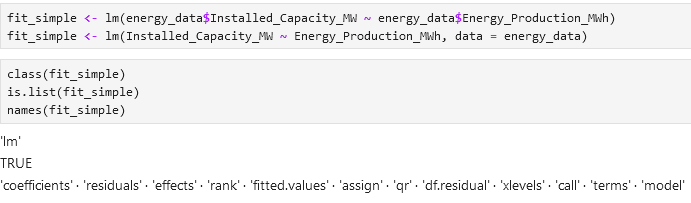
\includegraphics[width=1\linewidth]{lab1/obraz.png}
    \caption{Otrzymane drzewo}
    \label{fig:enter-label}
\end{figure}

Mimo to, spróbujmy wykonać kolejne procedury.

Sprawdźmy błąd testowy drzewa za pomocą metody zbioru walidacyjnego:

\begin{Rcode}
set.seed(1)
n <- nrow(energy_dataH)
train <- sample(n, n / 2)
test <- -train
reduction_height_tree <- tree(reduction ~ . - Air_Pollution_Reduction_Index, data = energy_dataH, subset = train)
tree_class <- predict(reduction_height_tree, newdata = energy_dataH[test,], type = "class")
table(tree_class, energy_dataH$reduction[test])
mean(tree_class != energy_dataH$reduction[test])
\end{Rcode}

Użycie drzewa do tak prostego zadania nie powoduje błędów:

\begin{figure}[H]
    \centering
    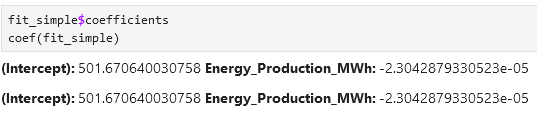
\includegraphics[width=1\linewidth]{lab5/obraz2.png}
    \caption{Enter Caption}
    \label{fig:enter-label}
\end{figure}

Skonstruujmy ciąg poddrzew:

\begin{Rcode}
set.seed(1)
reduction_high_cv <- cv.tree(reduction_height_tree, FUN = prune.misclass)
reduction_high_cv
plot(reduction_high_cv$size, reduction_height_tree$dev, type = "b")
\end{Rcode}

\begin{figure}[H]
    \centering
    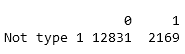
\includegraphics[width=1\linewidth]{lab5/obraz3.png}
    \caption{Parametry ciągu poddrzew}
    \label{fig:enter-label}
\end{figure}

Optymalizacja drzewa:

\begin{Rcode}
size_opt <- reduction_high_cv$size[which.min(reduction_high_cv$dev)]
reduction_high_pruned <- prune.misclass(reduction_height_tree, best = size_opt)
plot(reduction_high_pruned)
text(reduction_high_pruned, pretty = 0)
\end{Rcode}

Oczywiście wcześniej otrzymane drzewo jest już optymalne,

Dla testowy dla optymalnego drzewa:

\begin{Rcode}
pruned_class <- predict(reduction_high_pruned, newdata = energy_dataH[test,], 
                        type = "class")
table(pruned_class, energy_dataH$reduction[test])
mean(pruned_class != energy_dataH$reduction[test])
\end{Rcode}

Błąd testowy nadal jest równy 0.

\subsection{Drzewa regresyjne}
Kolejne drzewa mogą napotkać podobne problemy. Spróbujmy stworzyć drzewo regresyjne:

\begin{Rcode}
reductionv_tree <- tree(GHG_Emission_Reduction_tCO2e ~ ., data = energy_data)
\end{Rcode}

Szacujemy błąd testowy metodą zbioru walidacyjnego:

\begin{Rcode}
set.seed(1)
n <- nrow(energy_data)
train <- sample(n, n / 2)
test <- -train
reductionv_tree <- tree(GHG_Emission_Reduction_tCO2e ~ ., data = energy_data, subset = train)
reduction_pred <- predict(reductionv_tree, newdata = energy_data[test,])
mean((reduction_pred - energy_data$GHG_Emission_Reduction_tCO2e[test])^2)
\end{Rcode}

Otrzymaliśmy błąd testowy 12980682.

Wyznaczamy optymalne poddrzewo:
\begin{Rcode}
reduction_cv <- cv.tree(reductionv_tree)
plot(production_cv$size, production_cv$dev, type = "b")
\end{Rcode}

\begin{figure}[H]
    \centering
    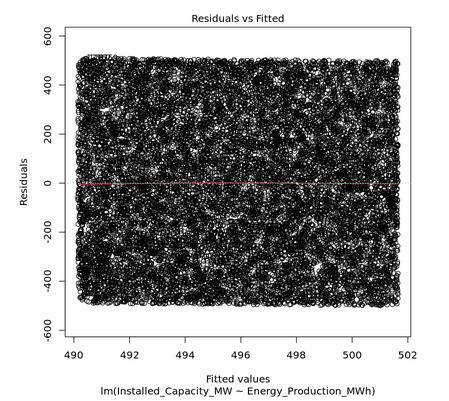
\includegraphics[width=1\linewidth]{lab5/obraz4.png}
    \caption{Zależność wielkości błędu od wielkości drzewa}
    \label{fig:enter-label}
\end{figure}

Przycinanie drzewa:
\begin{Rcode}
reduction_pruned <- prune.tree(reductionv_tree, best = 4)
\end{Rcode}

Dla optymalnego drzewa o 4 liściach, otrzymujemy błąd na poziomie 5183682

\subsection{Bagging i lasy losowe}
\subsubsection{Bagging}
Wykonajmy teraz bagging:

\begin{Rcode}
reduction_bag <- randomForest(GHG_Emission_Reduction_tCO2e ~ ., data = energy_data_clean, mtry = 4, importance = TRUE)
\end{Rcode}

Wygenerowaliśmy w ten sposób 500 drzew.

\begin{figure}[H]
    \centering
    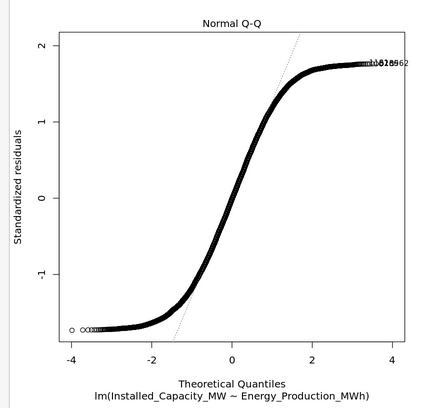
\includegraphics[width=1\linewidth]{lab5/obraz5.png}
    \caption{Dane o wygenerowanych drzewach}
    \label{fig:enter-label}
\end{figure}

\begin{figure}[H]
    \centering
    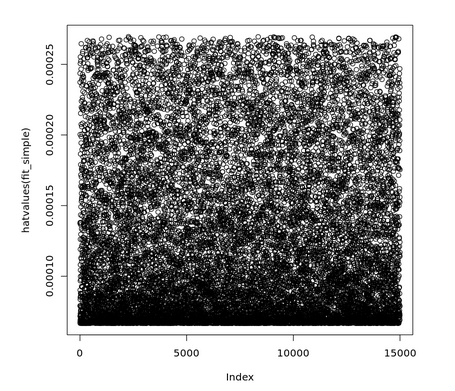
\includegraphics[width=1\linewidth]{lab5/obraz6.png}
    \caption{Ilość drzew a wartość błędu}
    \label{fig:enter-label}
    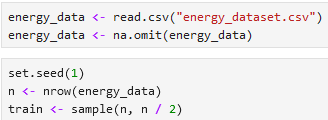
\includegraphics[width=1\linewidth]{lab5/obraz7.png}
    \caption{Ważność predyktorów}
    \label{fig:enter-label}
    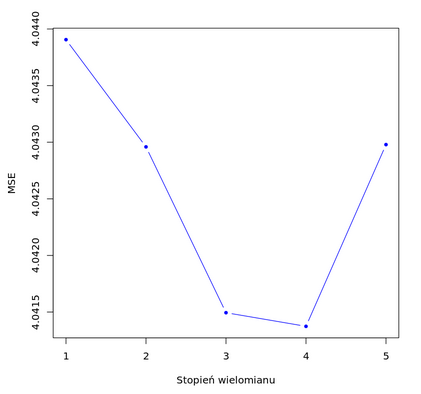
\includegraphics[width=1\linewidth]{lab5/obraz8.png}
    \caption{Ważność predyktorów}
    \label{fig:enter-label}
\end{figure}

Wyznaczmy błąd na zbiorze testowym:

\begin{Rcode}
set.seed(2)
production_bag <- randomForest(GHG_Emission_Reduction_tCO2e ~ ., data = energy_data_clean, subset = train, mtry = 4, importance = TRUE)
production_bag <- predict(production_bag, newdata = energy_data_clean[test,])
mean((production_bag - energy_data_clean$GHG_Emission_Reduction_tCO2e[test])^2)
\end{Rcode}

Otrzymaliśmy MSE na poziomie 209643854 - podobny rząd wielkości, co ostatnio. Ważność predyktorów nie uległa zmianie.

\begin{figure}[H]
    \centering
    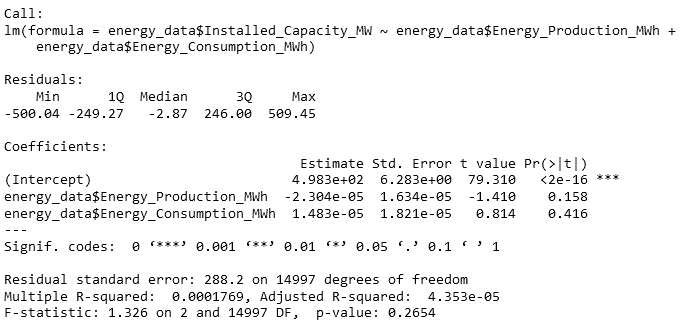
\includegraphics[width=1\linewidth]{lab5/obraz9.png}
    \caption{Ważność predyktorów.}
    \label{fig:enter-label}
\end{figure}

\subsubsection{Lasy losowe}
Teraz użyjmy lasów losowych:

\begin{Rcode}
set.seed(2)
reduction_rf <- randomForest(GHG_Emission_Reduction_tCO2e ~ ., data = energy_data_clean, subset = train,
                         importance = TRUE)
reduction_pred_rf <- predict(reduction_rf, newdata = energy_data_clean[test,])
mean((reduction_pred_rf - energy_data_clean$GHG_Emission_Reduction_tCO2e[test])^2)
\end{Rcode}

Otrzymaliśmy MSE równe 209643854.

Wazność predyktorów wygląda podobnie do poprzednich wyników:

\begin{figure}[H]
    \centering
    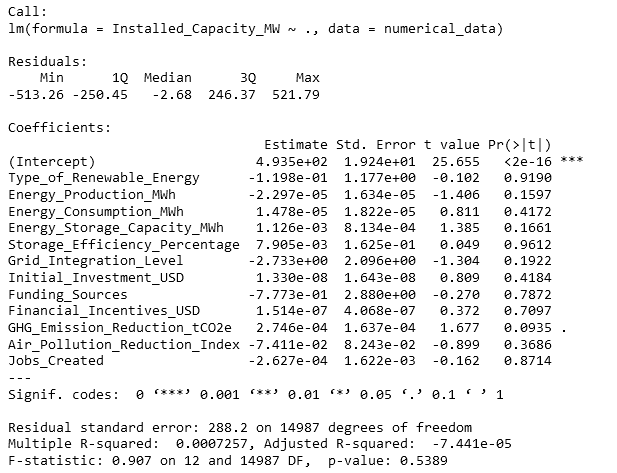
\includegraphics[width=1\linewidth]{lab5/obraz10.png}
    \caption{Wazność predyktorów}
    \label{fig:enter-label}
\end{figure}

Porównanie baggingu i lasu losowego:

\begin{figure}[H]
    \centering
    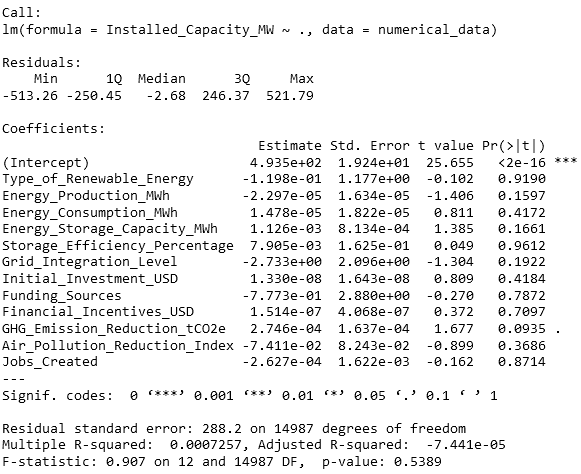
\includegraphics[width=1\linewidth]{lab5/obraz11.png}
    \caption{Las losowy z baggingiem (niebiesckie) i bez (czerwone).}
    \label{fig:enter-label}
\end{figure}

\subsection{Boosting}
Na koniec spróbujmy wykorzystać \textbf{boosting} do poprawienia wyników. W tym celu wykorzystamy bibliotekę \textbf{xgboost}:

\begin{Rcode}
data(energy_data_clean)
X <- as.matrix(energy_data_clean[, !names(energy_data_clean) %in% "GHG_Emission_Reduction_tCO2e"]) 
y <- energy_data_clean$GHG_Emission_Reduction_tCO2e

params <- list(
  objective = "reg:squarederror",  
  max_depth = 4,                   
  eta = 0.01,                      
  nthread = 2                      
)

nrounds <- 5000

reduction_boost <- xgboost(data = X, label = y, params = params, nrounds = nrounds, verbose = 0)
\end{Rcode}

Na ostatnich etapach tej metody otrzymaliśmy dużo lepsze wyniki niż wcześniej - aż o \textbf{dwa rzędy wielkości}:

\begin{figure}[H]
    \centering
    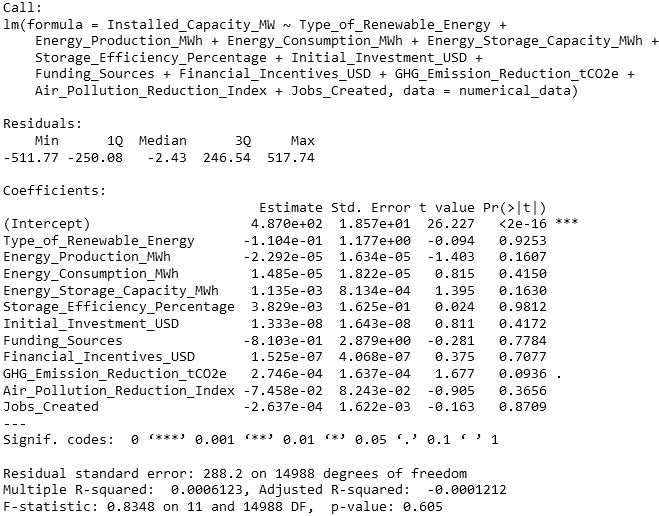
\includegraphics[width=1\linewidth]{lab5/obraz12.png}
    \caption{Dużo lepsze MSE osiągnięte przy pomocy boostingu}
    \label{fig:enter-label}
\end{figure}

Ważność predyktorów:
TODO

MSE na zbiorze walidacyjnym:
\begin{Rcode}
set.seed(2)

train <- sample(1:nrow(energy_data_clean), nrow(energy_data_clean) * 0.8)  
test <- setdiff(1:nrow(energy_data_clean), train)  

X_train <- as.matrix(energy_data_clean[train, !names(energy_data_clean) %in% "GHG_Emission_Reduction_tCO2e"])  
y_train <- energy_data_clean$GHG_Emission_Reduction_tCO2e[train]

X_test <- as.matrix(energy_data_clean[test, !names(energy_data_clean) %in% "GHG_Emission_Reduction_tCO2e"])  
y_test <- energy_data_clean$GHG_Emission_Reduction_tCO2e[test]

params <- list(
  objective = "reg:squarederror",  
  max_depth = 4,                   
  nthread = 2                     
)

nrounds <- 5000

reduction_boost <- xgboost(data = X_train, label = y_train, params = params, nrounds = nrounds, verbose = 0)

reduction_pred_boost <- predict(reduction_boost, newdata = X_test)

mse <- mean((reduction_pred_boost - y_test)^2)
\end{Rcode}

Otrzymaliśmy MSE o wartości 47907.

Dla $\lambda$ = 0.01:
\begin{Rcode}
params <- list(
  objective = "reg:squarederror",  
  max_depth = 4,                   
  eta = 0.01,                     
  nthread = 2                     
)

reduction_boost <- xgboost(data = X_train, label = y_train, params = params, nrounds = nrounds, verbose = 0)
reduction_pred_boost <- predict(reduction_boost, newdata = X_test)
mse <- mean((reduction_pred_boost - y_test)^2)
\end{Rcode}

MSE trochę lepsze - 41516.

Dla \textbf{d} (głębokości) = 1:
\begin{Rcode}
params <- list(
  objective = "reg:squarederror",  
  max_depth = 1,                   ,                    
  nthread = 2                     
)

reduction_boost <- xgboost(data = X_train, label = y_train, params = params, nrounds = nrounds, verbose = 0)
reduction_pred_boost <- predict(reduction_boost, newdata = X_test)
mse <- mean((reduction_pred_boost - y_test)^2)
\end{Rcode}

W tym przypadku MSE znacznie wzrosło - mamy 219684.
